% !TEX root = lac.tex
\section{Introduction}
\label{intro}

Due to the recent developments of gigantic social networks (e.g., Flickr, Facebook, and Twitter), the topic of {\it attributed graphs} has attracted attention from industry and research communities~\cite{attr-topic-sigmod2012,keyword-icde2002,keyword-icde2007,keyword-sigmod2007,keyword-vldb2005,keyword-yu-2009,keyword-vldb2011,fang2014}.  An attributed graph is essentially a graph associated with text strings or keywords.  Figure~\ref{fig:motivation} illustrates an attributed graph, where each vertex represents a social network user, and its keywords describe the interest of that user.

\begin{figure}
	\small
	\centering
	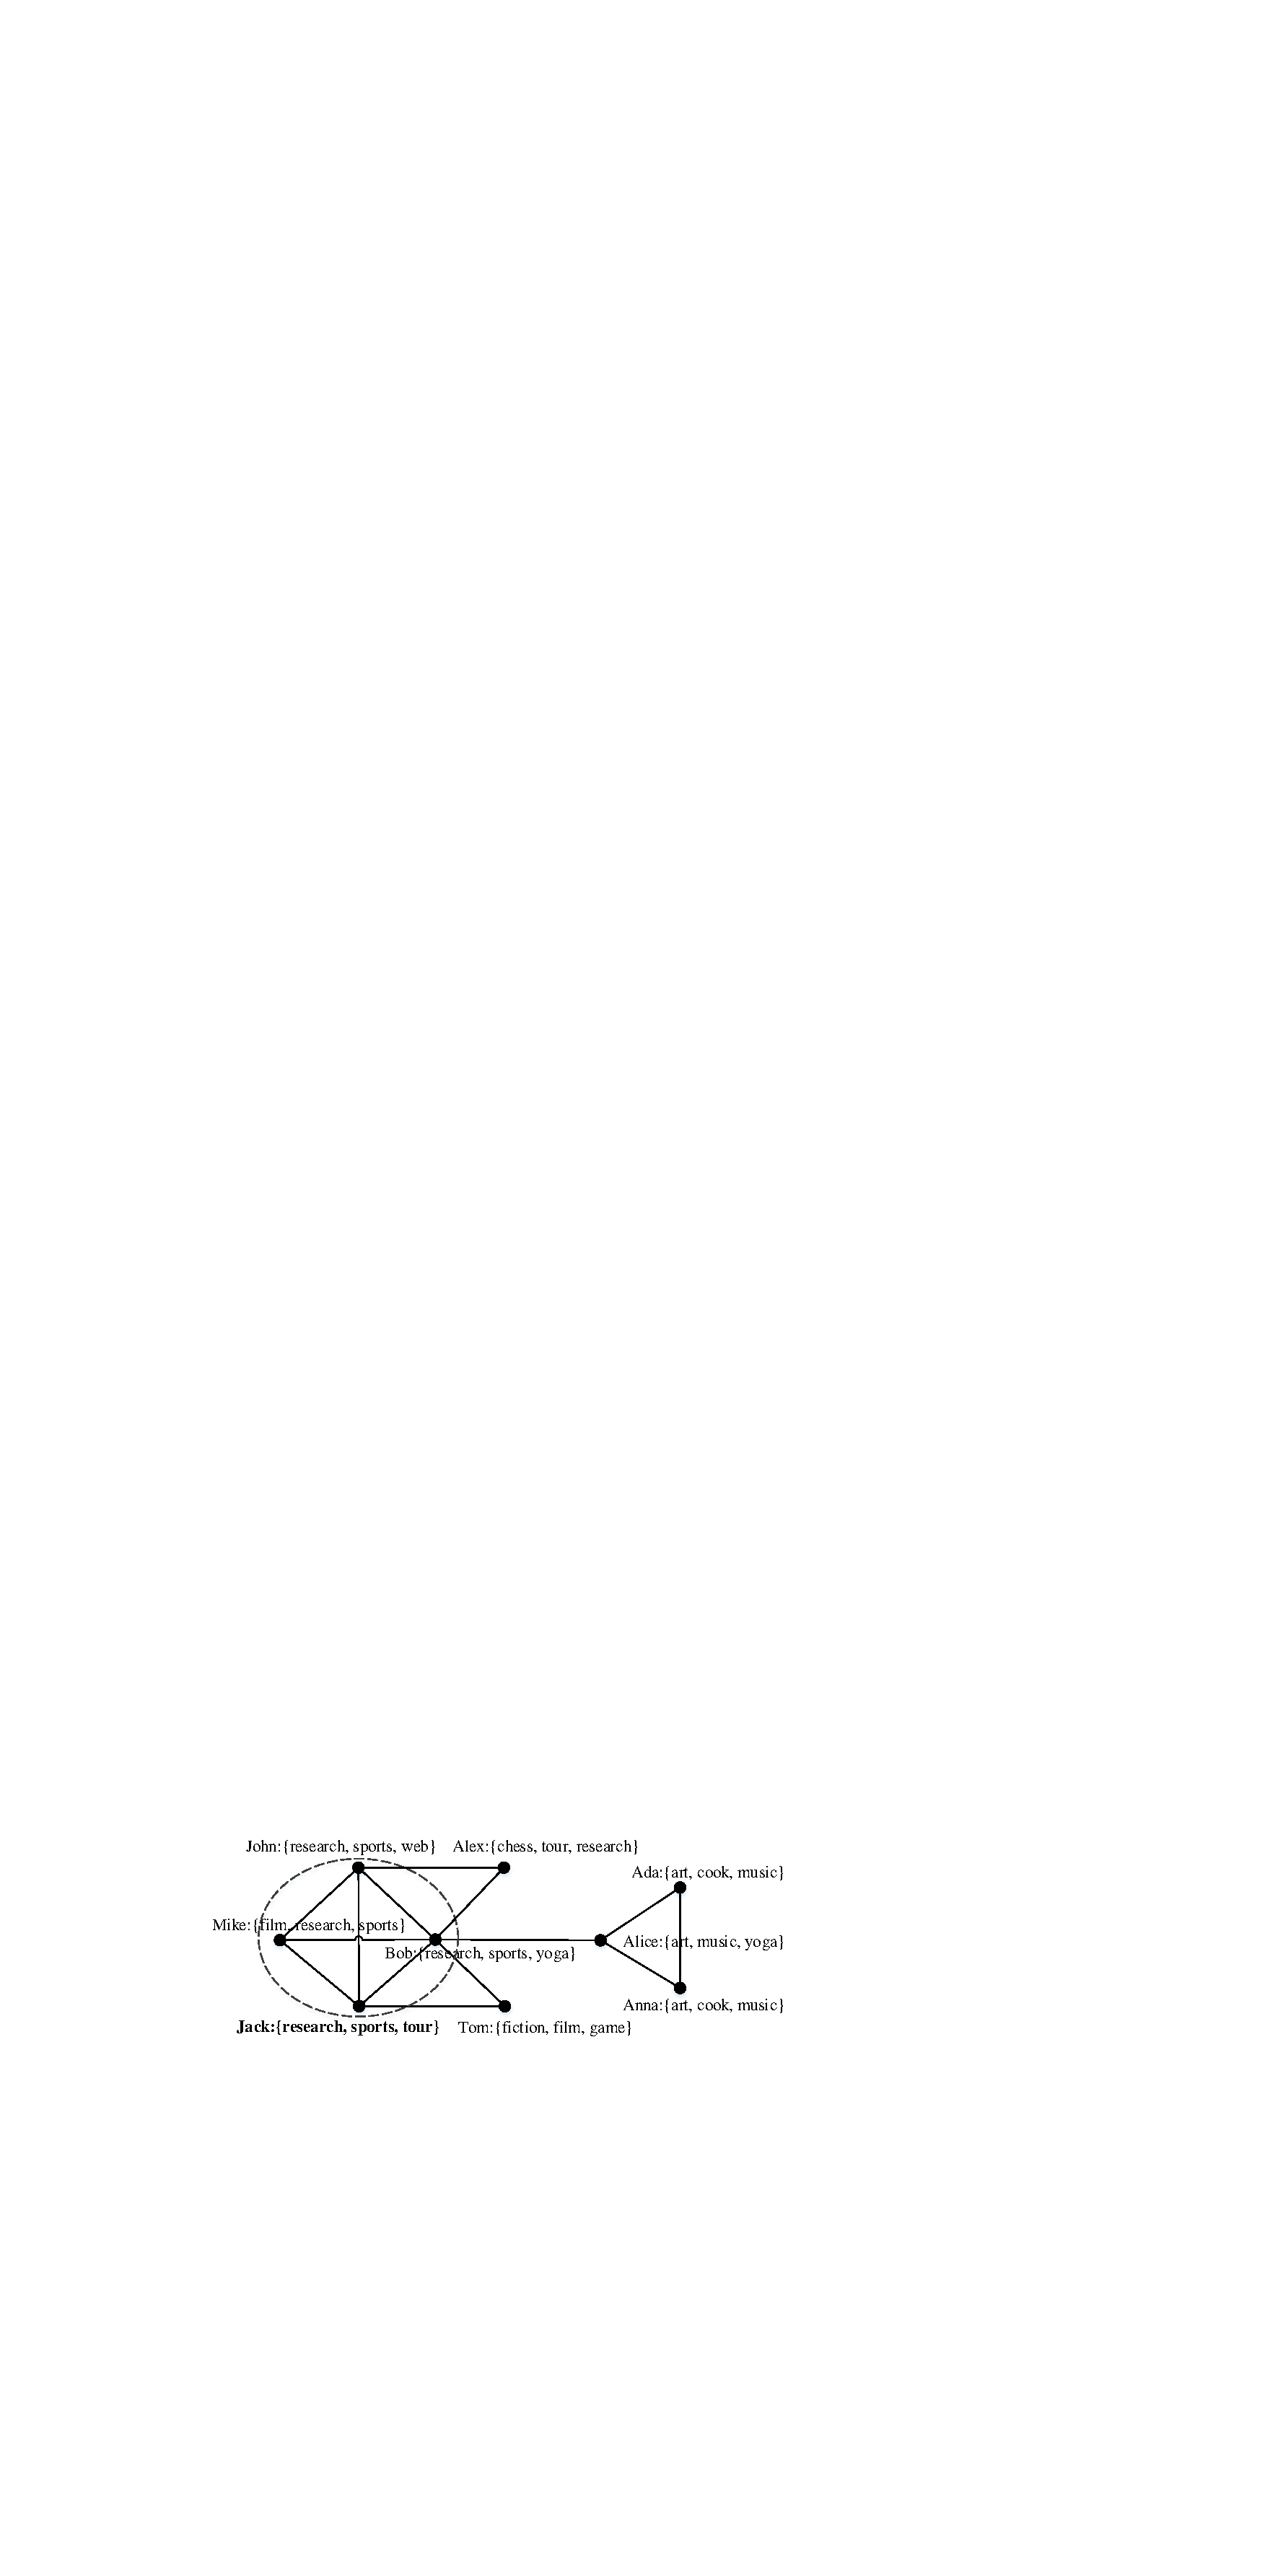
\includegraphics[width=0.88\linewidth]{figures/motivation}
	\caption{Attributed graph and AC (circled).}
	\label{fig:motivation}
\end{figure}

In this paper, we investigate the {\it attributed community query} (or ACQ). Given an attributed graph $G$ and a vertex $q \in G$, the ACQ returns one or more subgraphs of $G$ known as {\it attributed communities} (or ACs).  An AC is a kind of {\it community}, which consists of vertices that are closely related~\cite{KDD2010,local2014,online-sigmod2013,k-truss2014,community-phy2004,community-phy2010}.  Particularly, an AC satisfies {\it structure cohesiveness} (i.e., its vertices are closely linked to each other) and {\it keyword cohesiveness} (i.e., its vertices have keywords in common). Figure~\ref{fig:motivation} illustrates an AC (circled), which is a connected subgraph with vertex degree 3; its vertices $\{${\tt Jack}, {\tt Bob}, {\tt John}, {\tt Mike}$\}$ have two keywords (i.e., ``research'' and ``sports'') in common.

{\bf Prior works.} %An AC is a kind of {\it community}.
The problems related to retrieving communities from a graph can generally be classified into {\it community detection} (CD) and {\it community search} (CS).  In general, CD algorithms aim to retrieve all communities for a graph~\cite{community-phy2004,community-phy2010,attr-vldb2009,attr-topic-kdd2008,attr-topic-icml2009,attr-topic-sigmod2012,attr-www2013}. These solutions are not ``query-based'', i.e., they are not customized for a query request (e.g., a user-specified query vertex).
%For example, it is not clear how these algorithms can return a community that contain a given vertex $q$.
Moreover, they can take a long time to find all the communities for a large graph, and so they are not suitable for quick or {\it online} retrieval of communities. To solve these problems, CS solutions have been recently developed~\cite{KDD2010,local2014,online-sigmod2013,k-truss2014}. These approaches are query-based, and are able to derive communities in an ``online'' manner. However, existing CS algorithms assume {\it non-attributed} graphs, and only use the graph structure information to find communities. The ACQ is a class of CS problem for attributed graphs. As we will show, the use of keyword information can significantly improve the effectiveness of the communities retrieved. Table~\ref{tab:method} summarizes some representative existing works in this area.

\begin{table}
  \centering \footnotesize \caption {Classification of works in community retrieval. }\label{tab:method}
  \begin{tabular}{c|c|c}
     \hline
        \tabincell{c}{\textbf{Graph}\\ \textbf{Type}}
                       & \tabincell{c}{\textbf{Community}\\ \textbf{detection (CD)}}
                       & \tabincell{c}{\textbf{Community}\\ \textbf{search (CS)}}\\
     \hline\hline
        Non-attributed & \cite{community-phy2004,community-phy2010}
                       & \cite{KDD2010,local2014,online-sigmod2013,k-truss2014,vldb2015}\\
     \hline
        Attributed     & \cite{attr-vldb2009,attr-topic-kdd2008,attr-topic-icml2009,attr-topic-sigmod2012,attr-www2013}
                       & {\bf ACQ (This paper)} \\
     \hline
  \end{tabular}
\end{table}

{\bf Features of ACs.} We now present more details about ACs.

\noindent $\bullet$ {\bf Ease of interpretation.}
As demonstrated in Figure~\ref{fig:motivation}, an AC contains tightly-connected vertices with similar contexts or backgrounds. Thus, an ACQ user can focus on the common keywords or features of these vertices (e.g., the vertices of the AC in this example contain ``research'' and ``sports'', reflecting that all members of this AC like research and sports).  We call the set of common keywords among AC vertices
the \emph{AC-label}. In our experiments, the AC-labels facilitate understanding of the vertices that form the AC.

The design of ACs allows it to be used in setting up of social events. For example, if a Twitter member has many keywords about traveling (e.g., he posted a lot of photos about his trips, with keywords), issuing an ACQ with this member as the query vertex may return other members interested in traveling,  because their vertices also have keywords related to traveling. A group tour can then be recommended to these members.

\noindent $\bullet$ {\bf Personalization.}  The user of an ACQ can control the semantics of the AC, by specifying a set of $S$ of keywords. Intuitively, $S$ decides the meaning of the AC based on the user's need.  If we let $q$={\tt Jack}, $k$=2 and $S$=$\{$``research''$\}$,  the AC is formed by
$\{${\tt Jack}, {\tt Bob}, {\tt John}, {\tt Mike}, {\tt Alex}$\}$, who are all interested in research.
Let us consider another example in the DBLP bibliographical network, where each vertex's attribute is represented by the top-20 frequent keywords in their publications. Let $q$={\tt Jim} {\tt Gray}. If $S$ is the set of keywords \{transaction, data, management, system, research\}, we obtain the AC in Figure~\ref{fig:jim}(a), which contains six prominent database researchers closely related to Jim. On the other hand, when $S$ is \{sloan, digital, sky, survey, SDSS\}, the ACQ yields another AC in Figure~\ref{fig:jim}(b), which indicates the seven scientists involved in the SDSS project~\footnote{URL of the SDSS project: \url{http://www.sdss.org}.}.  Thus, with the use of different keyword sets $S$, different ``personalized'' communities can be obtained.

Existing CS algorithms, which do not handle attributed graphs, may not produce the two ACs above. For example, the CS algorithm in \cite{KDD2010} returns the community with {\it all} the 14 vertices shown in Figures~\ref{fig:jim}(a) and (b). The main reasons are: (1) these vertices are heavily linked with Jim; and (2) the keywords are not considered. In contrast, the use of set $S$ in the ACQ places these vertices into two communities, containing vertices that are cohesive in terms of {\it structure} and {\it keyword}. This allows a user to focus on the important vertices that are related to $S$. For example, using the AC of Figure~\ref{fig:jim}(a), a database conference organizer can invite speakers who have a close relationship with Jim.

The personalization feature is also useful in marketing. Suppose that Mary, a yoga lover, is a customer of a gym. An ACQ can be issued on a social network, with Mary as the query vertex and $S$=$\{$``yoga''$\}$. Since members of the AC contain the keyword ``yoga'', they can be the gym's advertising targets. On the other hand, current CS algorithms may return a community that contains one or more vertices without the keyword ``yoga''. It is not clear whether the corresponding user of this vertex is interested in yoga.

\noindent $\bullet$ {\bf Online evaluation.}  Similar to other CS solutions, we have developed efficient ACQ algorithms for large graphs, allowing ACs to be generated quickly upon a query request. On the contrary, existing CD algorithms~\cite{attr-vldb2009,attr-www2013,attr-topic-kdd2008,attr-topic-icml2009} that generate all communities for a graph are often considered to be offline solutions, since they are often costly and time-consuming, especially on very large graphs.

{\bf Technical challenges and our contributions.}
We face two important questions: (1) What should be a sound definition of an AC? (2) How to evaluate ACQ efficiently?  For the first question, we define an AC based on the {\it minimum degree}, which is one of the most common structure cohesiveness metrics~\cite{community-phy2004,community-phy2010,KDD2010,local2014}. This measure requires that every vertex in the community has a degree of $k$ or more.
%one of the most fundamental characteristics of graphs, and some recent works~\cite{KDD2010,local2014} have shown that it is better than many other metrics like average degree and density of a graph.
We formulate the keyword cohesiveness as maximizing the number of shared keywords in keyword set $S$. The shared keywords naturally reveal the common features among vertices (e.g., common interest of social network users). We can also use these shared keywords to explain how a community is formed.

\begin{figure}[ht]
    \centering
    \mbox{
        \subfigure[$S$=\{transaction, data, management, system, research\}]{
            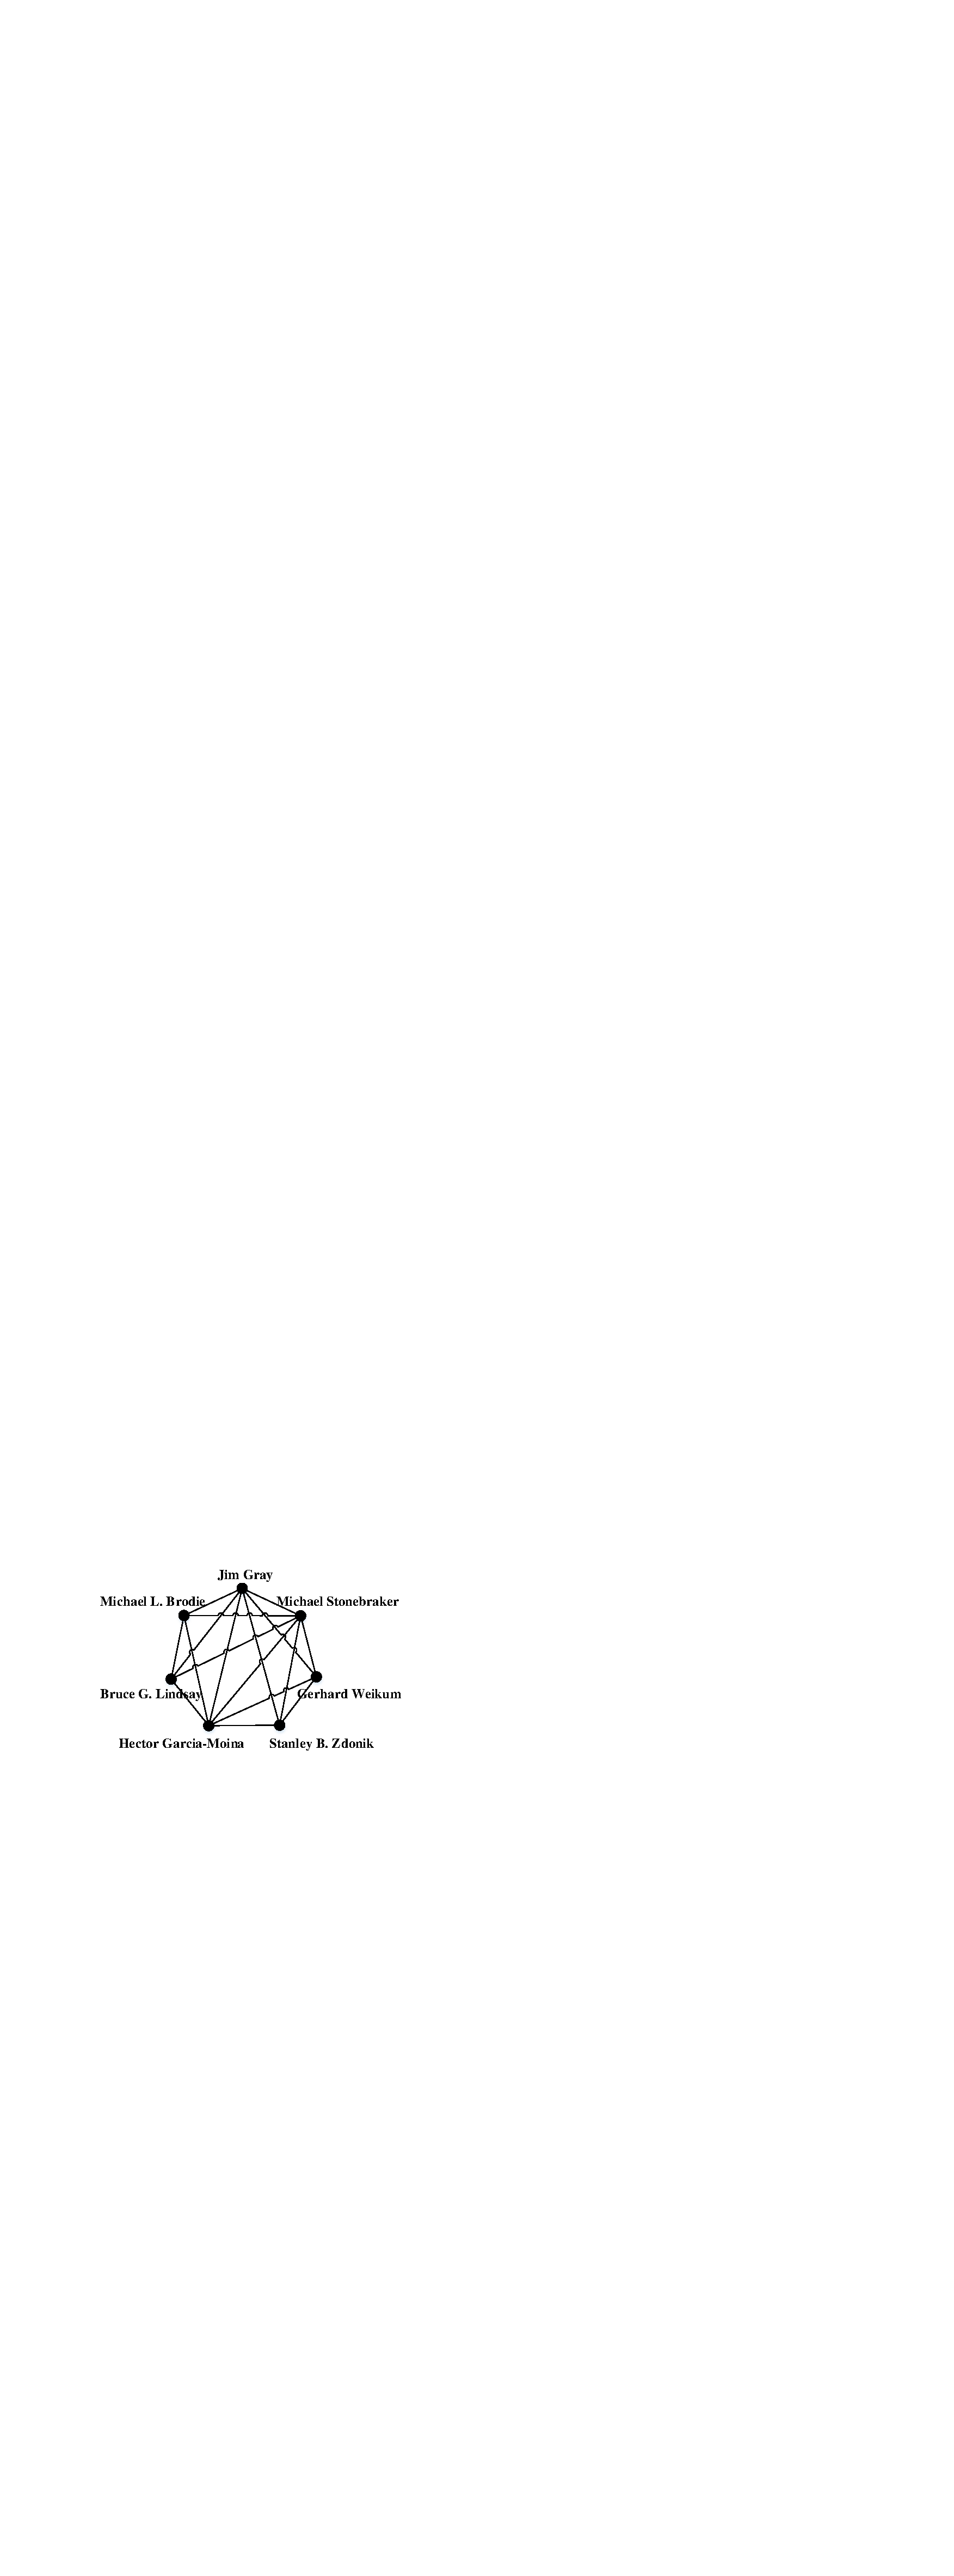
\includegraphics[width=.44\columnwidth]{figures/jim1}
            \label{fig:jim1}
        }
        \hspace{1ex}
        \subfigure[$S$=\{sloan, digital, sky, data, sdss\}]{
            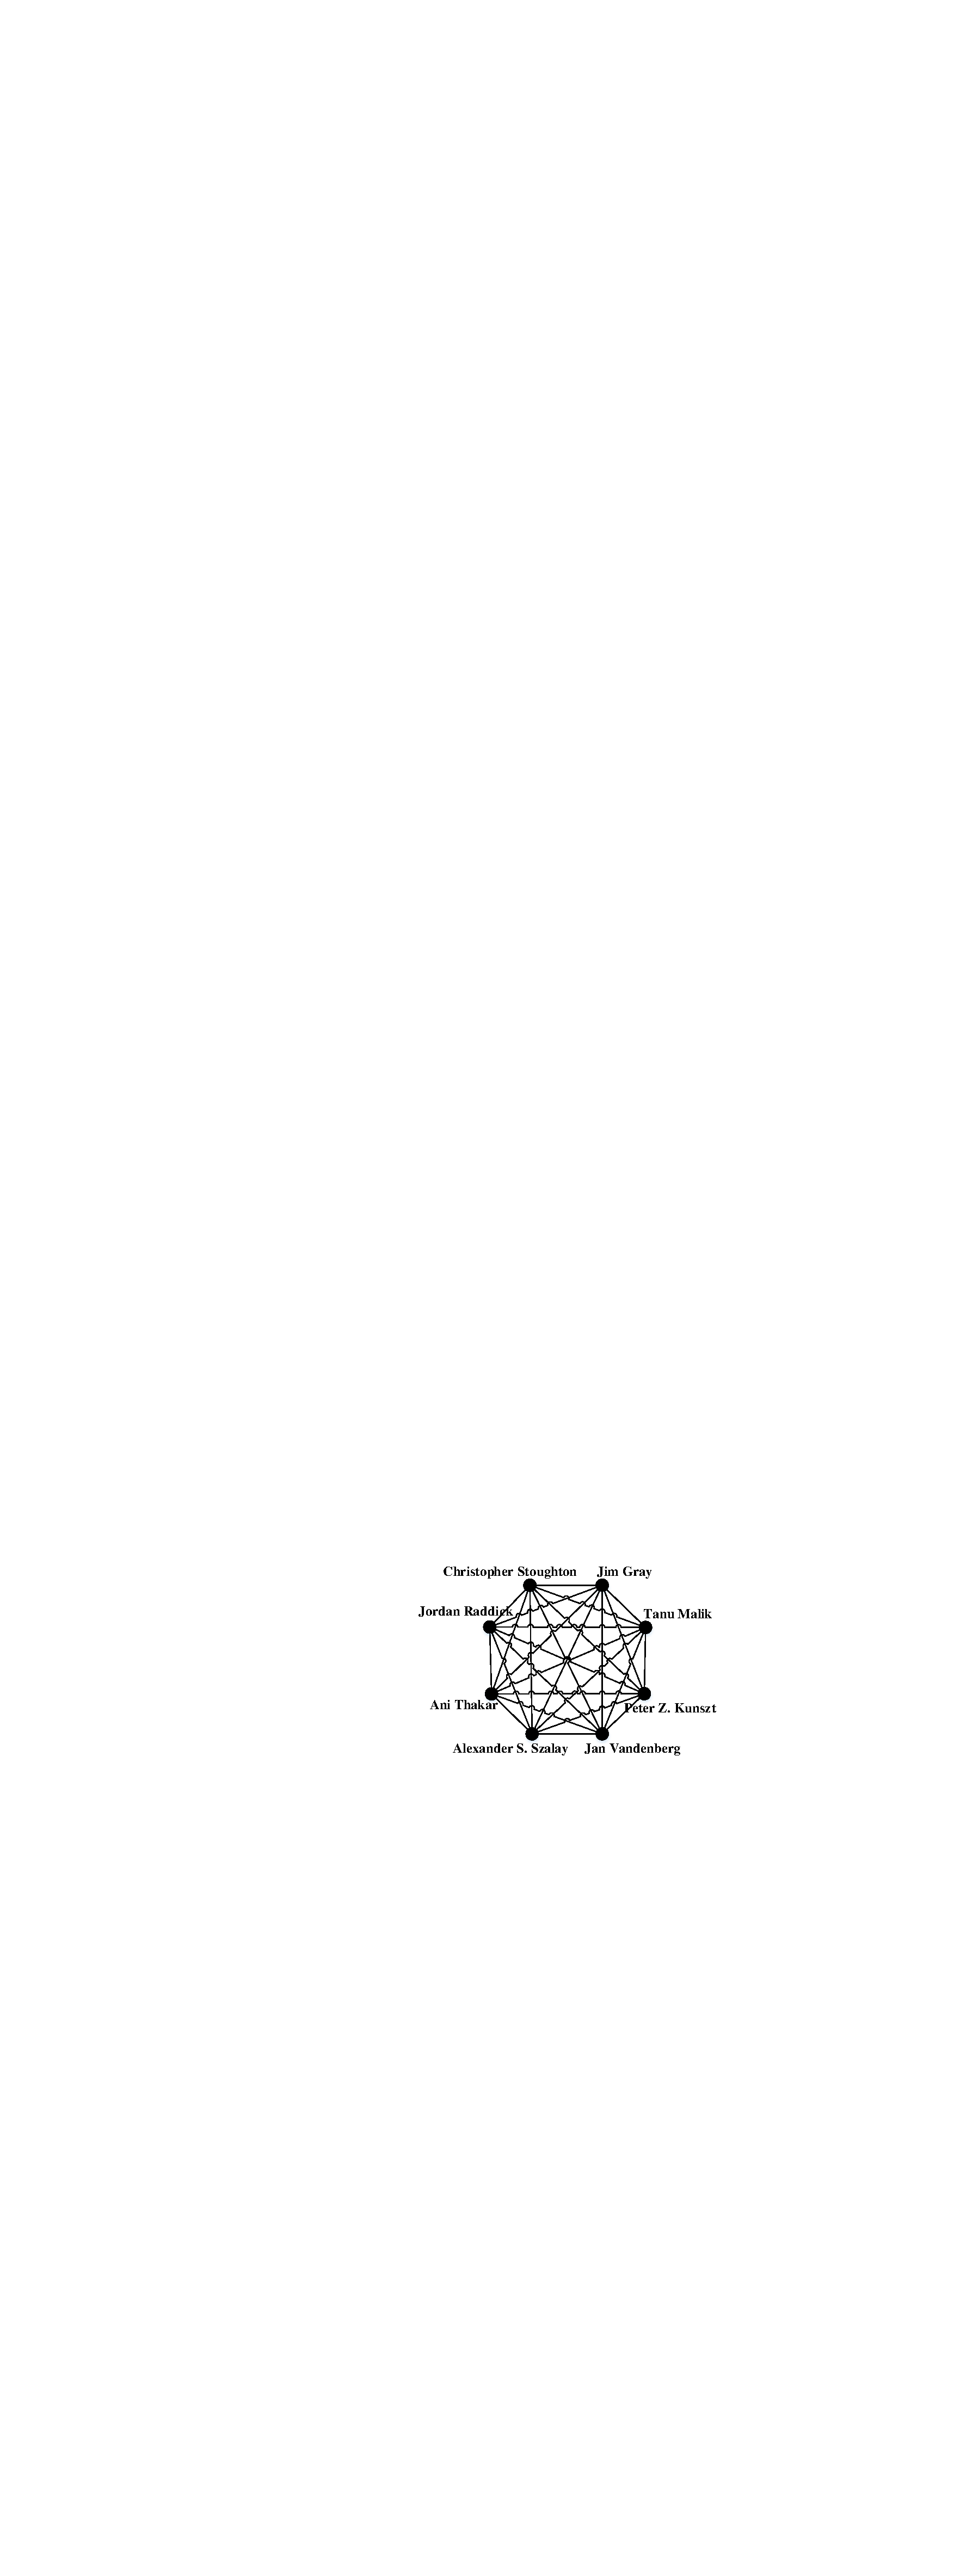
\includegraphics[width=.432\columnwidth]{figures/jim2}
            \label{fig:jim2}
        }
    }
    \caption{Two ACs of Jim Gray.}\label{fig:jim}
\end{figure}

The second question is not easy to answer, because the attributed graph $G$ to be explored can be very large, and the (structure and keyword) cohesiveness criteria can be complex to handle. A simple way is first to consider all the possible keyword combinations, and then return the subgraphs, which satisfy the minimum degree constraint and have the most shared keywords. This solution, which requires the enumeration of all the subsets of $q$'s keyword set, has a complexity exponential to the size $l$ of $q$'s keyword set. In our experiments, for some queries, $l$ can be up to 30, resulting in the consideration of $2^{30}=1,073,741,824$ subsets of $q$. The algorithm is impractical, especially when $q$'s keyword set is large.

We observe the {\it anti-monotonicity} property, which states that given a set $S$ of keywords, if it appears in every vertex of an AC, then for every subset $S'$ of $S$, there exists an AC in which every vertex contains $S'$. We use this intuition to propose better algorithms. We further develop the \emph{CL-tree}, an index that organizes the vertex keyword data in a hierarchical structure. The CL-tree has a space and construction time complexity linear to the size of $G$. We have developed three different ACQ algorithms based on the CL-tree, and they are able to achieve a superior performance.

We have performed extensive experiments on four large real graph datasets (namely Flickr, DBLP, Tencent, and DBpedia).
%{\color{red} We found that a large number of common keywords appear across vertices in our graph datasets. In DBLP, for instance, over 5,000 vertices share one keywords on average; over 700 vertices have two common keywords. Hence, using shared keywords among vertices as keyword cohesiveness makes sense.}
We found that a large number of common keywords appear across vertices in our graph datasets. In DBLP, for instance, an AC with one common keyword contains over 5,000 vertices on average; an AC with two common keywords contains over 700 vertices. Hence, using shared keywords among vertices as keyword cohesiveness makes sense.
We have also studied how to quantify the quality of a community, based on occurrence frequencies of keywords and similarity between the keyword sets of two vertices. We conducted a detailed case study on DBLP. These results confirm the superiority of the AC over the communities returned by existing community detection and community search algorithms, in terms of community quality. The performance of our best algorithm is 2 to 3 order-of-magnitude better than solutions that do not use the CL-tree. Another advantage of our approaches is that they organize and search vertex keywords for ACs effectively, achieving a higher efficiency than existing community search solutions (that do not use vertex keywords in the community search process).

%Note that although our solutions are developed based on the minimum degree metric, they can potentially be used to address other definitions of communities (e.g., $k$-truss).

{\bf Organization.} We review the related work in Section~\ref{related}, and define the ACQ problem formally in Section~\ref{problem}. Section~\ref{basic} presents the basic solutions, and Section~\ref{index} discusses the CL-tree index.
We present the query algorithms in Section~\ref{query}.
Our experimental results are reported in Section~\ref{experiment}.
We conclude in Section~\ref{conclusion}.


%%%%%%%%%%%%%%%%%%%%%%%
%{\color{red} Yixiang}


%p1: attributed graph & non-attributed graph
%In recent years, with the proliferation of rich information in online social networks (e.g., Flickr and Twitter), vertices in graphs are usually associated with attributes that describe the characteristics and properties of the vertices. This novel type of graphs is called \emph{attributed} graph~\cite{attr-topic-sigmod2012}. Figure~\ref{fig:motivation} shows a social network, in which each vertex's attribute is represented by three keywords. Analyzing both the links and attributes of attributed graphs has received plenty of research attentions, and enables many real applications. For example, Google indexes and ranks Web pages using both their links and contents. In this paper, we focus on finding communities from attributed graphs.

%p2: general introduction of community detection and community search
%Communities are prevalent in social networks, bibliographical graphs, and knowledge bases, and they enable emerging applications like product advertisement and setting up of social events. Finding communities from graph databases can power a lot of important applications, including friend recommendation, advertising, tag suggestion and setting up of social events.
%Detecting communities from a graph has been studied extensively~\cite{community-phy2004,community-phy2010}.
%Recently, there is another related but different problem, called~\emph{online community search}, has received plenty of research interest~\cite{KDD2010,local2014,online-sigmod2013,k-truss2014}. Given a query vertex in a graph $G$, the goal of community search is to find the best community related to the query vertex. It is a query-dependent variant of the community detection problem~\cite{KDD2010}. The main difference between these two problems is that community detection usually aims to identify all the communities from an entire graph by optimizing some pre-defined criterions, where the graph needs to be partitioned a-priori with no reference to query vertices, while community search is to find the most likely community that contains the query vertex~\cite{KDD2010}.

%\begin{figure}
%	\small
%	\centering
%	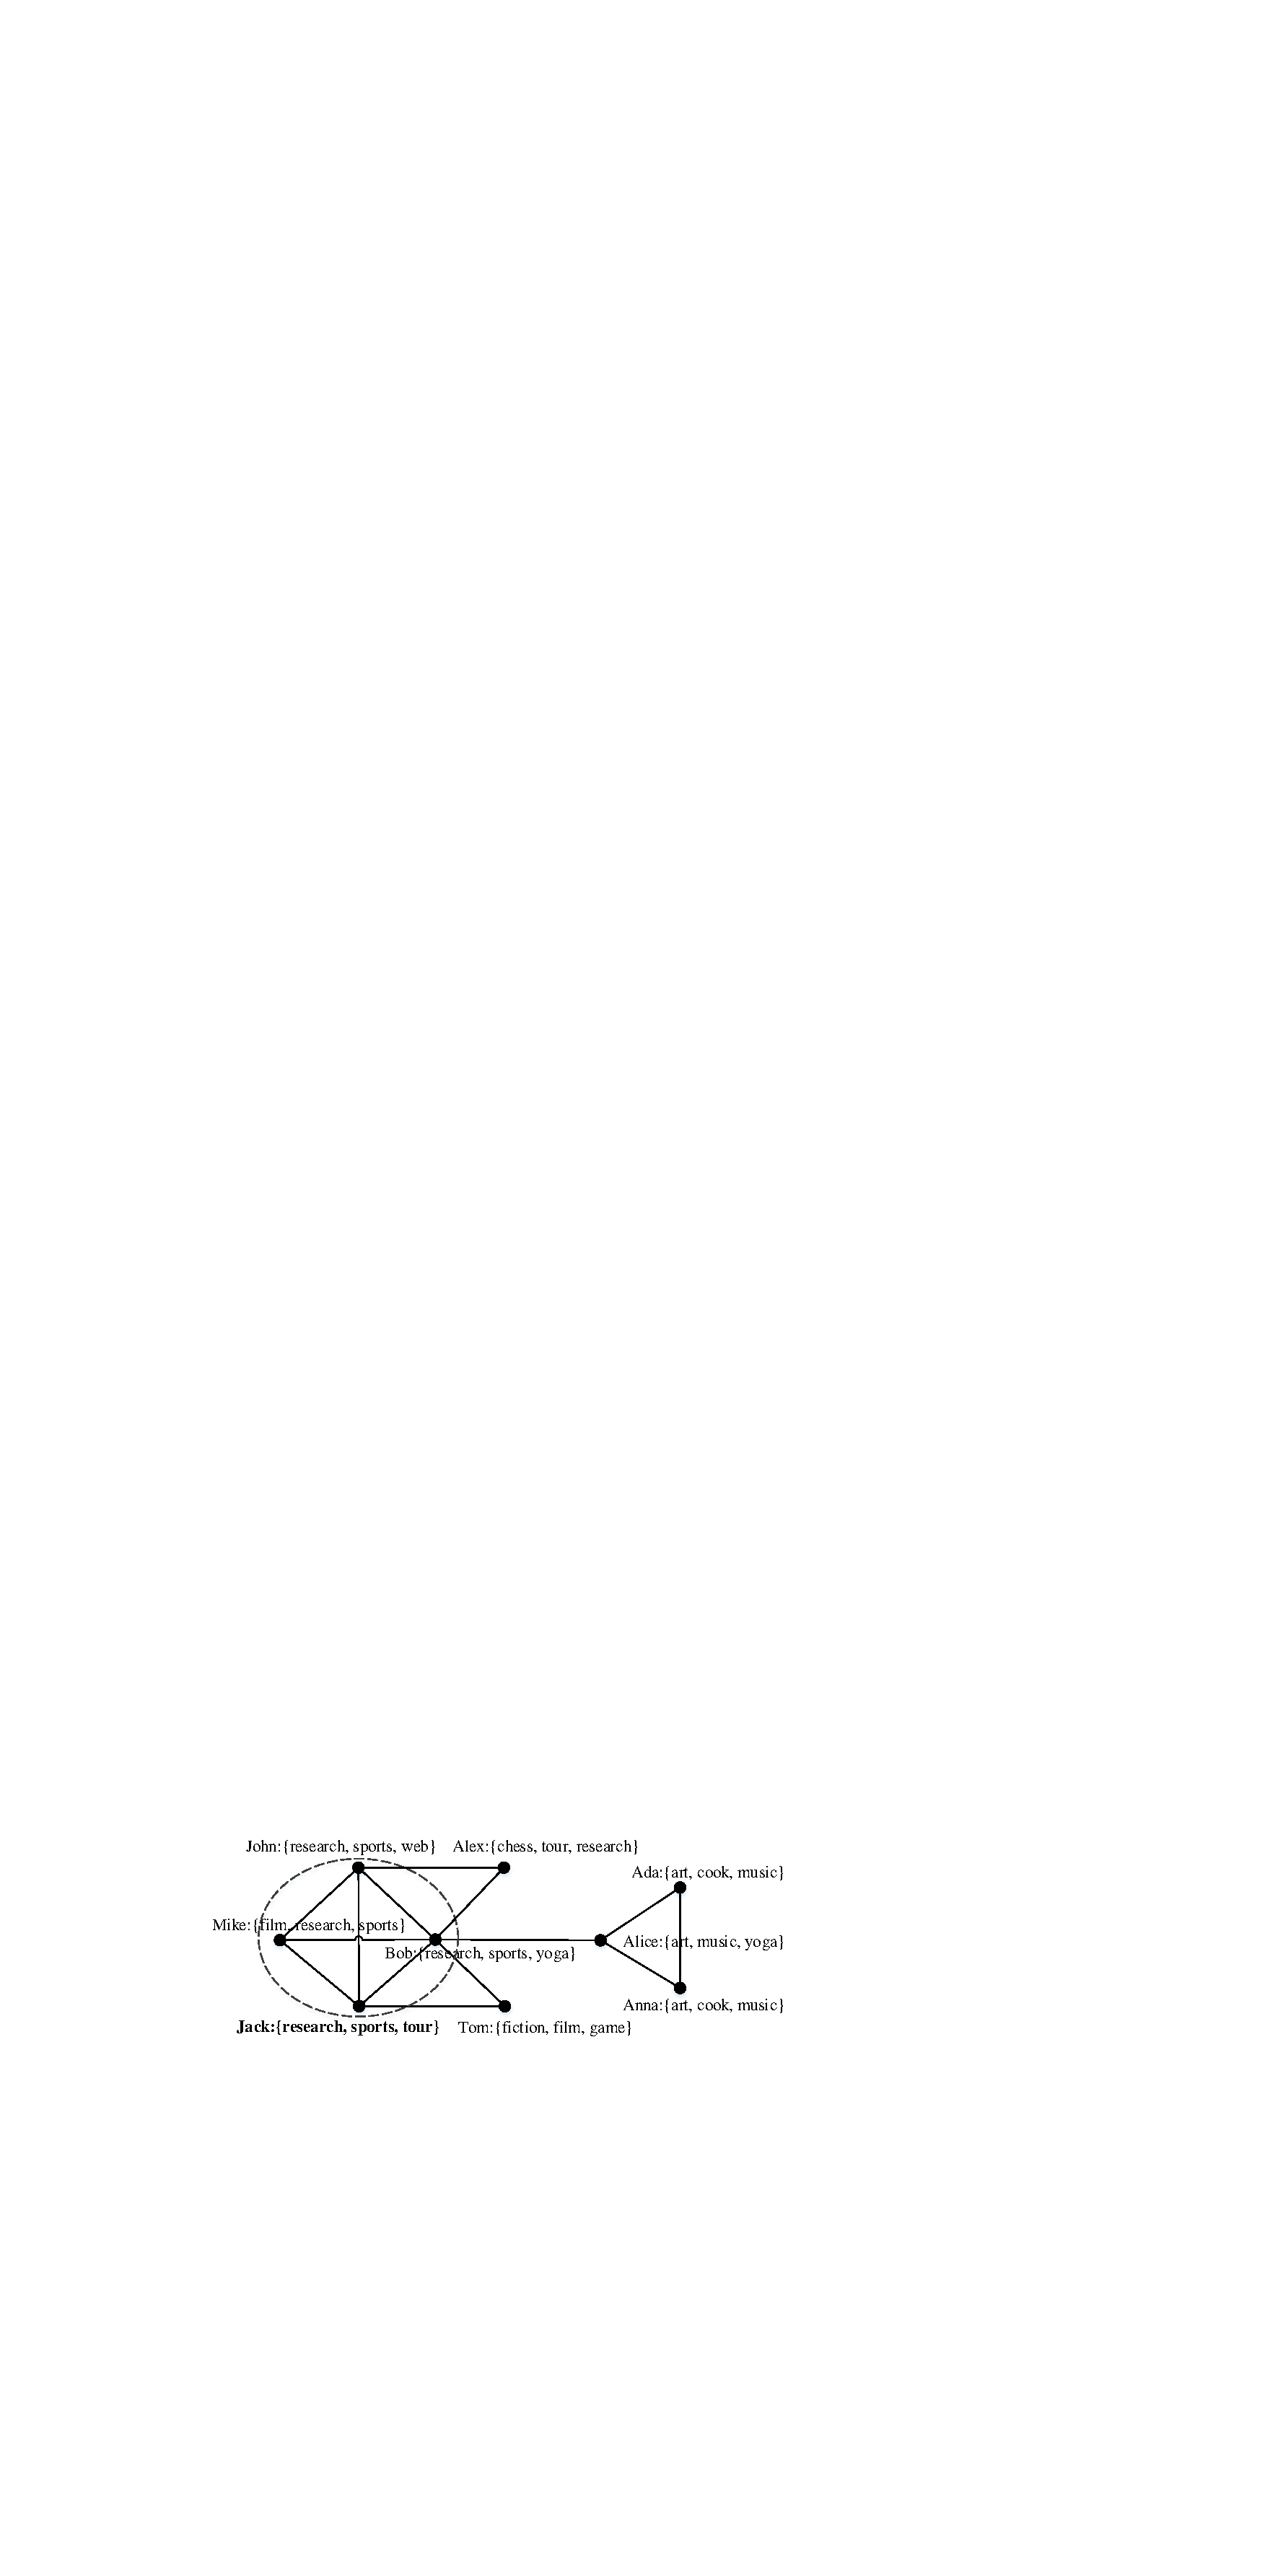
\includegraphics[width=0.88\linewidth]{figures/motivation}
%	\caption{Illustrating AC search.}
%	\label{fig:motivation}
%\end{figure}

%p3: introduce AC and its applications
%There are some existing works~\cite{attr-vldb2009,attr-topic-kdd2008,attr-topic-icml2009,attr-topic-sigmod2012,attr-www2013} on detecting communities from attributed graphs, but surprisingly little attention has been paid to online search of communities from attributed graphs. In this paper, we investigate how to search communities online from attributed graphs, where the attribute of each vertex is represented by a set of \emph{keywords}. We propose the {\it label-aware community} (or AC). Similar to the communities found by existing community detection/search algorithms, the AC is a subgraph of $G$ satisfies {\it structure cohesiveness} (i.e., the vertices involved in the AC are closely linked to each other). The AC also exhibits {\it keyword cohesiveness} (i.e., the vertices contained in the AC have keywords in common).
%An example AC for Figure~\ref{fig:motivation} is one that contains $\{${\tt Jack}, {\tt Bob}, {\tt John}, {\tt Mike}$\}$, which form a connected subgraph with vertex degree of 3, and have ``research'' and ``sports'' keywords in common. Essentially, an AC consists of vertices with similar contexts or backgrounds, allowing a query user to focus on the common features of these vertices. ACs can be useful in setting up of social events. For example, if a Twitter user has many keywords about traveling (e.g., he posted a lot of photos about his trips, with labels), an AC search about this user is likely to return people who are also interested in traveling (since their vertices have keywords related to traveling). A tour can then be organized for the people of the AC. Advertisement about traveling products (e.g., cameras and backpacks) can also be recommended to this AC.

%p4: the structure cohesiveness and keyword cohesiveness of AC
%We develop the notion of AC based on the structure cohesiveness metric {\it minimum degree}~\cite{community-phy2004, community-phy2010,KDD2010,local2014}, which requires that every vertex in the community has a degree of $k$ or more. We have studied several possible criteria for defining keyword cohesiveness (e.g., that the number of keywords shared by AC vertices is maximum, or each vertex's keyword set contains a user-given keyword set). The set of shared keywords in common by all members in an AC is called its \emph{label}. We further investigate the {\it AC search} problem: given a query vertex $q\in G$, the minimum degree $k$ and a set of keywords $S$, the goal is to find the ACs, which contain $q$ and have labels being a subset of $S$. In Figure~\ref{fig:motivation}, let $q$={\tt Jack}, $k$=2 and $S$ be {\tt Jack}'s keyword set. Then the AC returned is a subgraph that contains {\tt Jack}, {\tt Bob}, {\tt John} and {\tt Mike}, and its label is $\{$research, sports$\}$.

%p5: explain AC search on DBLP dataset
%Let us further illustrate the {\it AC search} on the DBLP bibliographical network, in which each vertex's attribute is represented by the top-20 frequent keywords in their publications. Let $q$={\tt Jim} {\tt Gray}, $k$=4 and $S$ be the set of his keywords. Figure~\ref{fig:jim} shows the two ACs found and their respective labels.  We can see that the two ACs contain completely different authors (except Jim himself). Moreover, the label of each AC reflects the backgrounds of the people within that AC (e.g., in Figure~\ref{fig:jim}(a), the 6 researchers connected to Jim are well known for their work in database systems; in Figure~\ref{fig:jim}(b), the 7 scientists linked to Jim are involved in the SDSS (or Sloan Digital Sky Survey) project)~\footnote{URL of the SDSS project: \url{http://www.sdss.org}.}.
%
%\begin{figure}[ht]
%    \centering
%    \mbox{
%        \subfigure[\{transaction, data, management, system, research\}]{
%            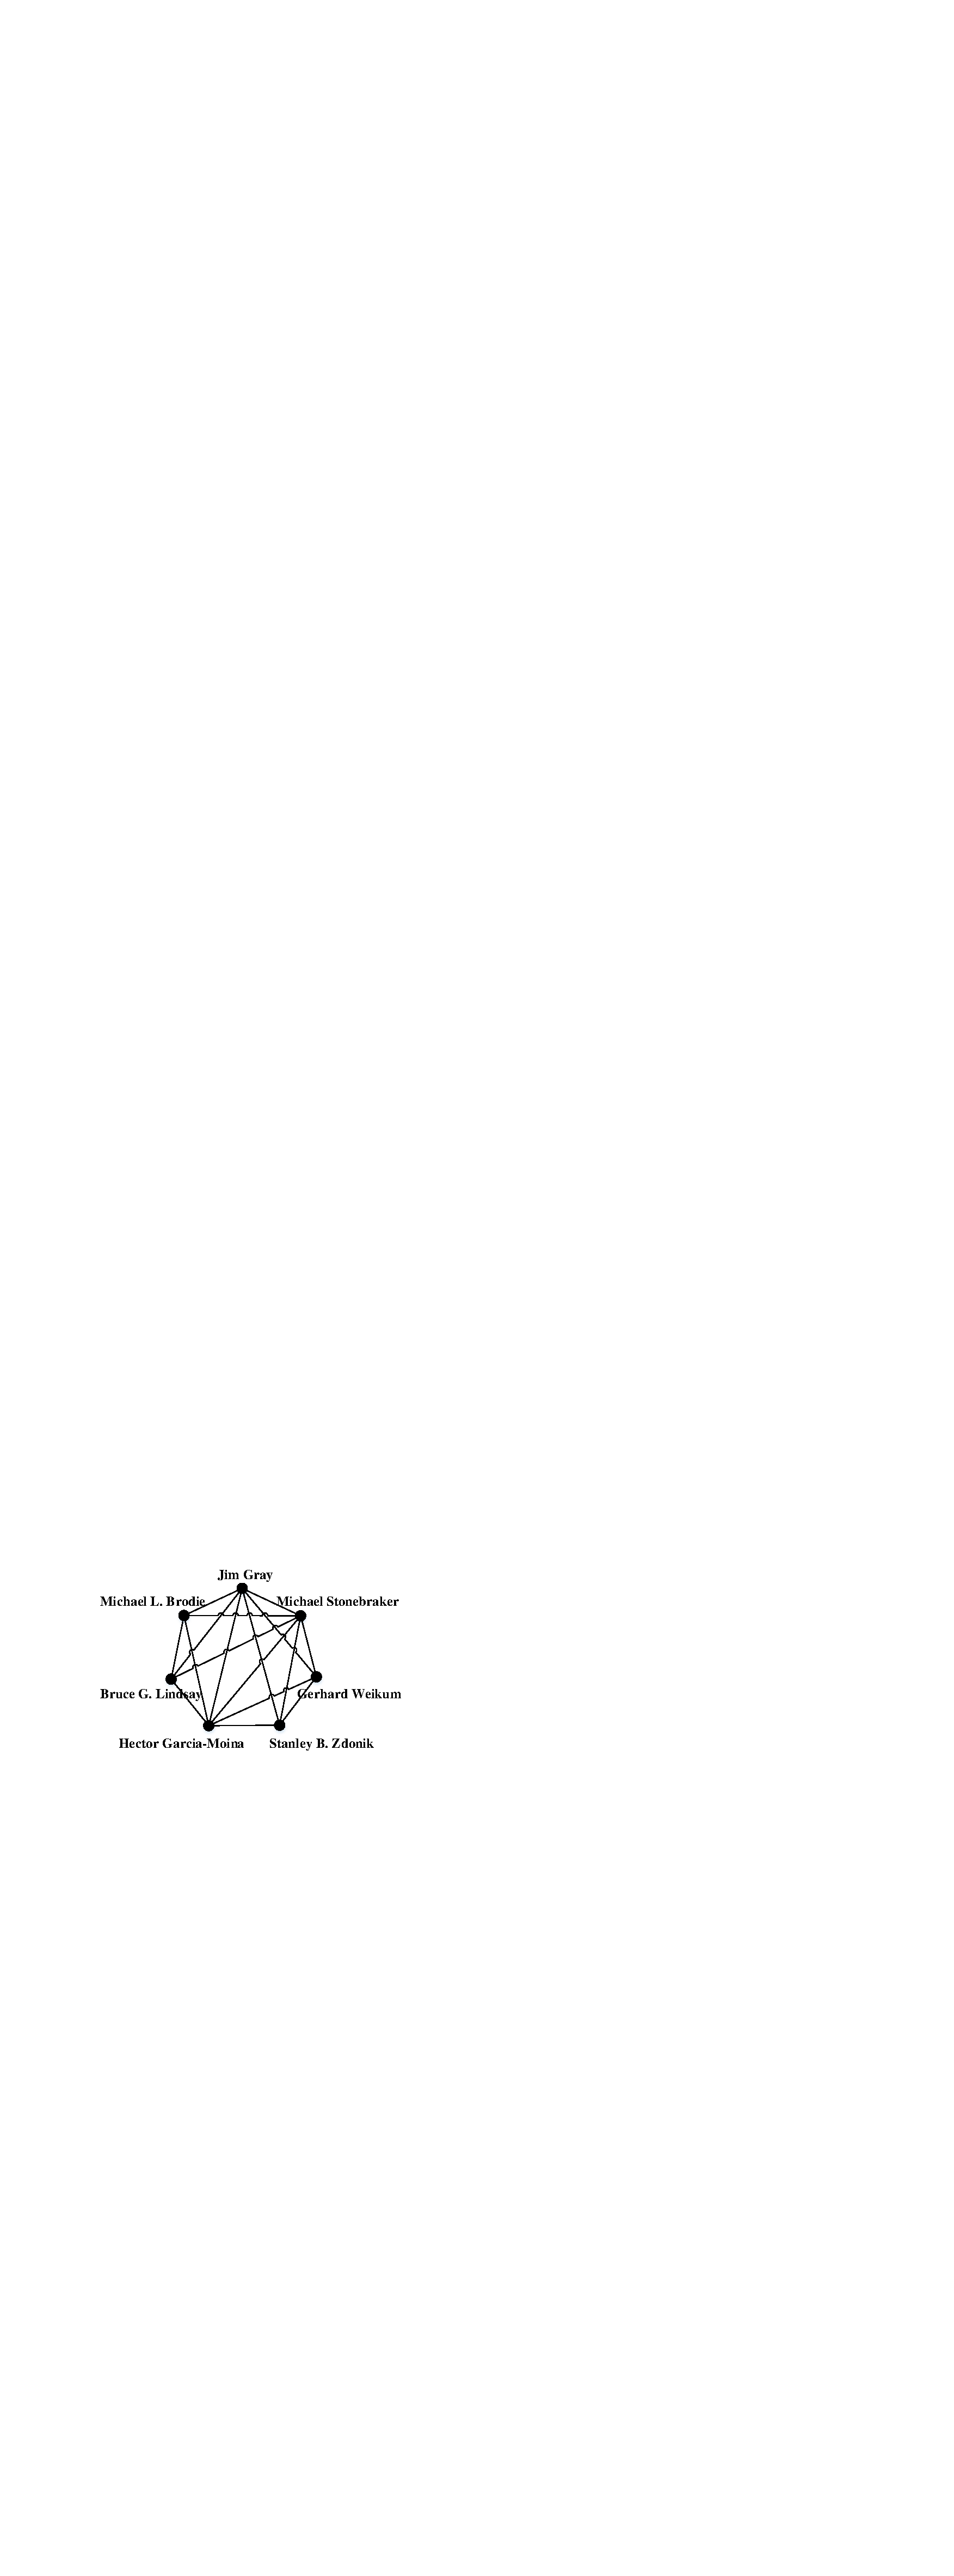
\includegraphics[width=.445\columnwidth]{figures/jim1}
%            \label{fig:jim1}
%        }
%        \hspace{1ex}
%        \subfigure[\{sloan, digital, sky, data, sdss\}]{
%            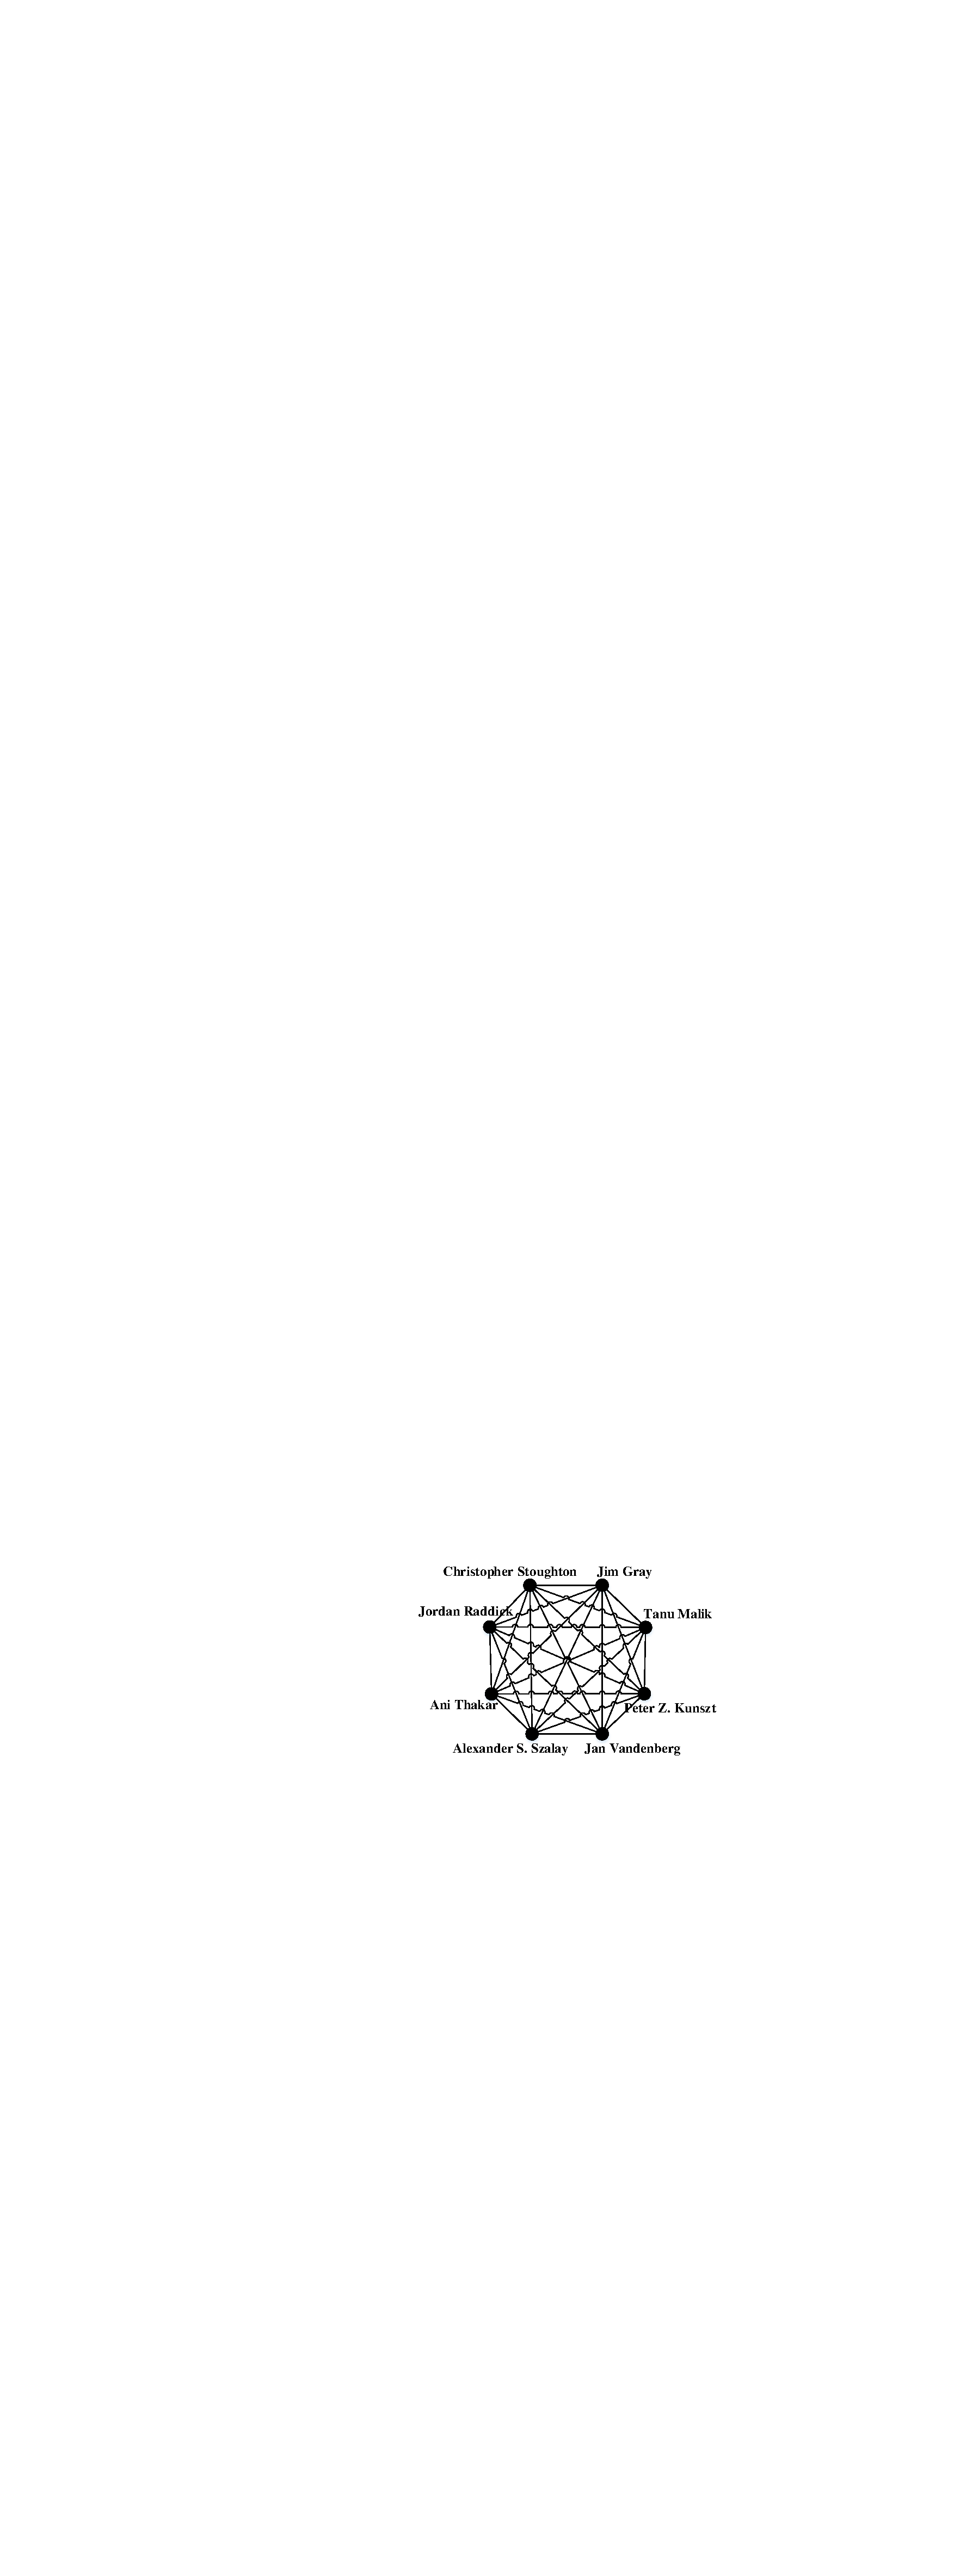
\includegraphics[width=.435\columnwidth]{figures/jim2}
%            \label{fig:jim2}
%        }
%    }
%    \caption{Two ACs of Jim Gray (with AC labels).}\label{fig:jim}
%\end{figure}

%p6: comparison with existing works on community detection
%Table~\ref{tab:method} lists some representative works on detecting and searching communities from non-attributed and attributed graphs. To support online search of communities from attributed graphs, a straightforward approach is to adapt existing community detection methods~\cite{attr-vldb2009,attr-topic-kdd2008,attr-topic-icml2009,attr-topic-sigmod2012,attr-www2013}
%by detecting all the communities in an offline pre-computing stage, and return the communities containing the query vertices. Compared with this approach, our online AC search has following advantages:

%$\bullet$ \emph{AC search is more personalized}. In Figure~\ref{fig:motivation}, existing methods~\cite{attr-vldb2009,attr-www2013} tend to partition the graph into two communities, which contains the left six persons and right three persons respectively. Let {\tt Jack} and {\tt Alex} be the query vertices. The adapted approach returns the same community for them, which contains a set $C_1$=$\{${\tt Jack}, {\tt Tom}, {\tt Bob}, {\tt John}, {\tt Mike}, {\tt Alex}$\}$. While AC search ($k$=2, $S$ is their keywords) finds two different communities for them, which contain sets $C_2$=$\{${\tt Jack}, {\tt Bob}, {\tt John}, {\tt Mike}$\}$ and $C_3$=$\{${\tt Jack}, {\tt Bob}, {\tt John}, {\tt Mike}, {\tt Alex}$\}$ respectively. Note that {\tt Tom} is not included, as he has no common interest with them.

%Moreover, as we can specify a set $S$ of keywords when performing AC search, we can control over the semantics of the ACs desired. This implies, even for the same query vertex, we can also find different communities by using different $S$.
%For example, if we let $q$={\tt Jack}, $k$=2 and $S$=$\{$``sports''$\}$, AC search returns $C_3$.

%$\bullet$ \emph{ACs are more easier to interpret}. The label, a set of shared keywords, of the AC explicitly explains the theme of the AC. For example, the label of $C_2$, i.e., $\{$research, sports$\}$, shows that all the users in this community may like research and sports. While for $C_1$, as {\tt Tom} share little common interest with other users, we cannot explain precisely why he is in this community.

%$\bullet$ \emph{AC search has better scalability}. It is costly, time-consuming and often unnecessary to find communities for an entire graph. For example, existing methods~\cite{attr-vldb2009,attr-www2013,attr-topic-kdd2008,attr-topic-icml2009} often need to consider the pairwise distance/similarity among vertices, which makes them unable to scale well on big graphs with million or even billion of vertices. In contrast, AC search just finds the communities of the query vertex online. Moreover, as AC search usually works on a subgraph, rather than an entire graph, it can be easily adapted for dynamic graphs.

%
%\begin{table}
%%  \centering \footnotesize \caption {Representative works on finding communities.}\label{tab:method}
%  \centering \footnotesize \caption {Classification of works in community retrieval. }\label{tab:method}
%  \begin{tabular}{c|c|c}
%     \hline
%        \tabincell{c}{\textbf{Graph}\\ \textbf{Type}}          & \tabincell{c}{\textbf{Community}\\ \textbf{detection (CD)}}
%                                    & \tabincell{c}{\textbf{Community}\\ \textbf{search (CS)}}\\
%     %\hline
%     %   {\bf Graph}    & \textbf{Com. discovery}
%     %                  & \textbf{Com. search}\\
%     \hline\hline
%        Non-attributed & \cite{community-phy2004,community-phy2010}
%                       & \cite{KDD2010,local2014,online-sigmod2013,k-truss2014,vldb2015}\\
%     \hline
%        Attributed     & \cite{attr-vldb2009,attr-topic-kdd2008,attr-topic-icml2009,attr-topic-sigmod2012,attr-www2013}
%                       & {\bf ACQ (This paper)} \\
%     \hline
%  \end{tabular}
%\end{table}

%p7: compare with existing community search works
%We notice that there are some existing community search methods~\cite{KDD2010,local2014,online-sigmod2013,k-truss2014,vldb2015}. But they mainly focus on non-attributed graph, so they cannot handle the vertices' attributes. For example, continue the previous query on the DBLP network ($q$={\tt Jim} {\tt Gray}, $k$=4 and $S$ be the set of his keywords). The existing algorithm~\cite{KDD2010} returns the community contains all the 14 vertices shown in Figures~\ref{fig:jim}(a) and (b). The main reasons are: (1) these vertices are heavily linked with Jim; and (2) the keywords are not considered.
%In contrast, the AC search places these vertices into two communities, containing vertices that are cohesive in terms of {\it structure} and {\it keyword}. The ACs found allow a user to focus on the important vertices that constitute a community. For example, using the AC of Figure~\ref{fig:jim}(a), a database conference organizer can invite speakers who have a close relationship to Jim.

%p8: challenges of AC search
%Performing an AC search is not straightforward, since the graph $G$ to be explored can be very large, and the (structure and keyword) cohesiveness criteria for governing the community search are complex. To tackle this challenge, a straightforward way is first to consider all the possible keyword combinations, and then return the subgraphs, which satisfy the minimum degree constraint and have the most shared keywords.
%However, this solution, which requires the enumeration of all the subsets of $q$'s keyword set, has a complexity exponential to the size $l$ of $q$'s keyword set. In our experimental evaluation, for some queries, $l$ can have a value of 30, resulting in the consideration of $2^{30}=1,073,741,824$ subsets of $q$. The algorithm is impractical, especially when $q$'s keyword set is large. We observe the {\it anti-monotonicity} property, which states that given a set $S$ of keywords, if it appears in every vertex of an AC, then for every subset $S'$ of $S$, there exists an AC in which every vertex contains $S'$.
%We use this intuition to propose better algorithms. We further develop the \emph{CL-tree}, an index that organizes the vertex keyword data in a hierarchical structure. The CL-tree has a space and construction time complexity linear to the size of $G$. We have developed three different AC search algorithms based on the CL-tree, and they are able to achieve a superior performance.
%
%We have performed extensive experiments on our solutions on four large real graph datasets (namely Flickr, DBLP, Tencent, and DBpedia). We have developed several measures to measure the quality of a community, based on occurrence frequencies of keywords and similarity between the keyword sets of two vertices. We conducted a detailed case study on DBLP. These results confirm the superiority of the AC over the communities returned by existing community detection and community search algorithms, in terms of community quality. The performance of our best algorithm is 2 to 3 order-of-magnitude better than solutions that do not use the CL-tree. Another advantage of our approaches is that they organize and search vertex keywords for ACs effectively, achieving a higher efficiency than existing community search solutions (that do not use vertex keywords in the community search process).
%
%As a summary, we propose the AC, which is a new definition of the community that considers both structure and keyword cohesiveness. To perform efficient AC search, we develop the CL-tree and its associated algorithms. We perform experimental evaluation on real graph datasets to validate our approaches.  Notice that although our solutions are developed based on the minimum degree metric in this paper, they can potentially be used to address other definitions of communities (e.g., $k$-truss).  Our study can also inspire the development of better community detection algorithms that take vertex keywords into account.
%
%The rest of our paper is organized as follows.
%We review the related work in Section~\ref{related}, and define the problem formally in Section~\ref{problem} and
%Section~\ref{basic} presents the basic solutions, and Section~\ref{index} discusses the CL-tree.
%We present the query algorithms in Section~\ref{query}.
%Our experimental results are reported in Section~\ref{experiment}.
%We conclude in Section~\ref{conclusion}.























%The old SIGMOD version is as follows:
\iffalse
The retrieval of {\it communities} from large graph databases, including social networks, bibliographical graphs, and knowledge bases, has received plenty of research interest.  Given a graph $G$, the \emph{community detection} problem is about the extraction of subgraph structures whose vertices are closely connected~\cite{community-phy2004,community-phy2010}. Another related problem, called {\it community search}, focuses on retrieving subgraph(s) from $G$ which have a close relationship with a given query vertex $q$~\cite{KDD2010,local2014,online-sigmod2013,k-truss2014}.
Community generation algorithms power a lot of important applications, including friend recommendation, advertising, tag suggestion and setting up of social events. Figure~\ref{fig:motivation} shows a social network, in which an edge with two vertices $u$ and $v$ represents a relationship between $u$ and $v$.
Given that $q$ is the vertex {\tt Jack}, and every vertex required for a community has a minimum degree of $k=2$, a possible community~\cite{KDD2010} of $q$ is the one that contains six vertices, namely {\tt Jack}, {\tt Mike}, {\tt John}, {\tt Bob}, {\tt Alice}, and {\tt Tom}.


Existing solutions often make use of the graph edge information to produce communities. However, they overlook the rich information associated with vertices, which is commonly found in large graph databases. In Twitter, for instance, a vertex contains a large number of keywords, describing the hobbies, education and check-in pACes of the user corresponding to the vertex. In Figure~\ref{fig:motivation}, {\tt Jack} has three keywords depicting his interest (e.g., ``research''). These keywords, which give information about the vertices involved, can be important to obtaining and explaining a community. Unfortunately, this is often not considered by existing algorithms, which may output communities with vertices that are not semantically close to each other. Let us consider the community of {\tt Jack} in Figure~\ref{fig:motivation} (circled) again.  We can see that the keywords associated with the vertices of this community span a wide range of topics (e.g., research, tour, yoga, and cook). But what is the main theme of this community? What are the members' common interest? Why do these people constitute to the community of {\tt Jack}? Notice that {\tt Bob} and {\tt Mike} are closely related to {\tt Jack}, since the keywords ``research'' and ``sports'' appear in their vertices (e.g., these three persons belong to the same research team and often play basketball together).  However, {\tt Jack} appears to be remote from {\tt Alice} and {\tt Tom}, because {\tt Jack} does not share any keywords with them (e.g., {\tt Tom} and {\tt Jack} are alumni but do not have a common keyword; {\tt Alice} is included into {\tt Jack}'s community simply because she is linked to {\tt Bob}). A better candidate for {\tt Jack}'s community could be the one that only contains {\tt Bob}, {\tt Mike}, and himself.

In this paper, we study how vertex keywords can be used to improve the search of communities. We propose the {\it label-aware community} (or AC). Similar to the communities found by traditional community detection/search algorithms, the AC is a subgraph of $G$ satisfies {\it structure cohesiveness} (i.e., the vertices involved in the AC are closely linked to each other). The AC also exhibits {\it keyword cohesiveness} (i.e., the vertices contained in the AC have keywords in common). An example AC for Figure~\ref{fig:motivation} is one that contains {\tt Jack}, {\tt Bob}, and {\tt Mike}, which form a connected subgraph with vertex degree of 2 or more, and have ``research'' and ``sports'' keywords in common. Essentially, an AC consists of vertices with similar contexts or backgrounds, allowing a query user to focus on the common features of these vertices. ACs can be useful in setting up of social events. For example, if a social network user has many keywords about traveling (e.g., he posted a lot of photos about his trips, with labels), an AC search about this user is likely to return people who are also interested in traveling (since their vertices have keywords related to traveling). A tour can then be organized for the people contained in the AC. Advertisement about traveling products (e.g., cameras and backpacks) can also be recommended to this AC. We develop the notion of AC based on the structure cohesiveness metric {\it minimum degree}~\cite{community-phy2004, community-phy2010,KDD2010,local2014}, which requires that every vertex in the community has a degree of $k$ or more.
We have studied several possible criteria for defining keyword cohesiveness (e.g., that the number of keywords shared by AC vertices is maximum, or each vertex's keyword set contains a user-given keyword set). We further investigate the {\it AC search} problem, which aims to find the AC(s) that contain(s) a given query vertex $q$.

\begin{figure}
    \centering
    \mbox{
        \subfigure[\{transaction, data, management, system, research\}]{
            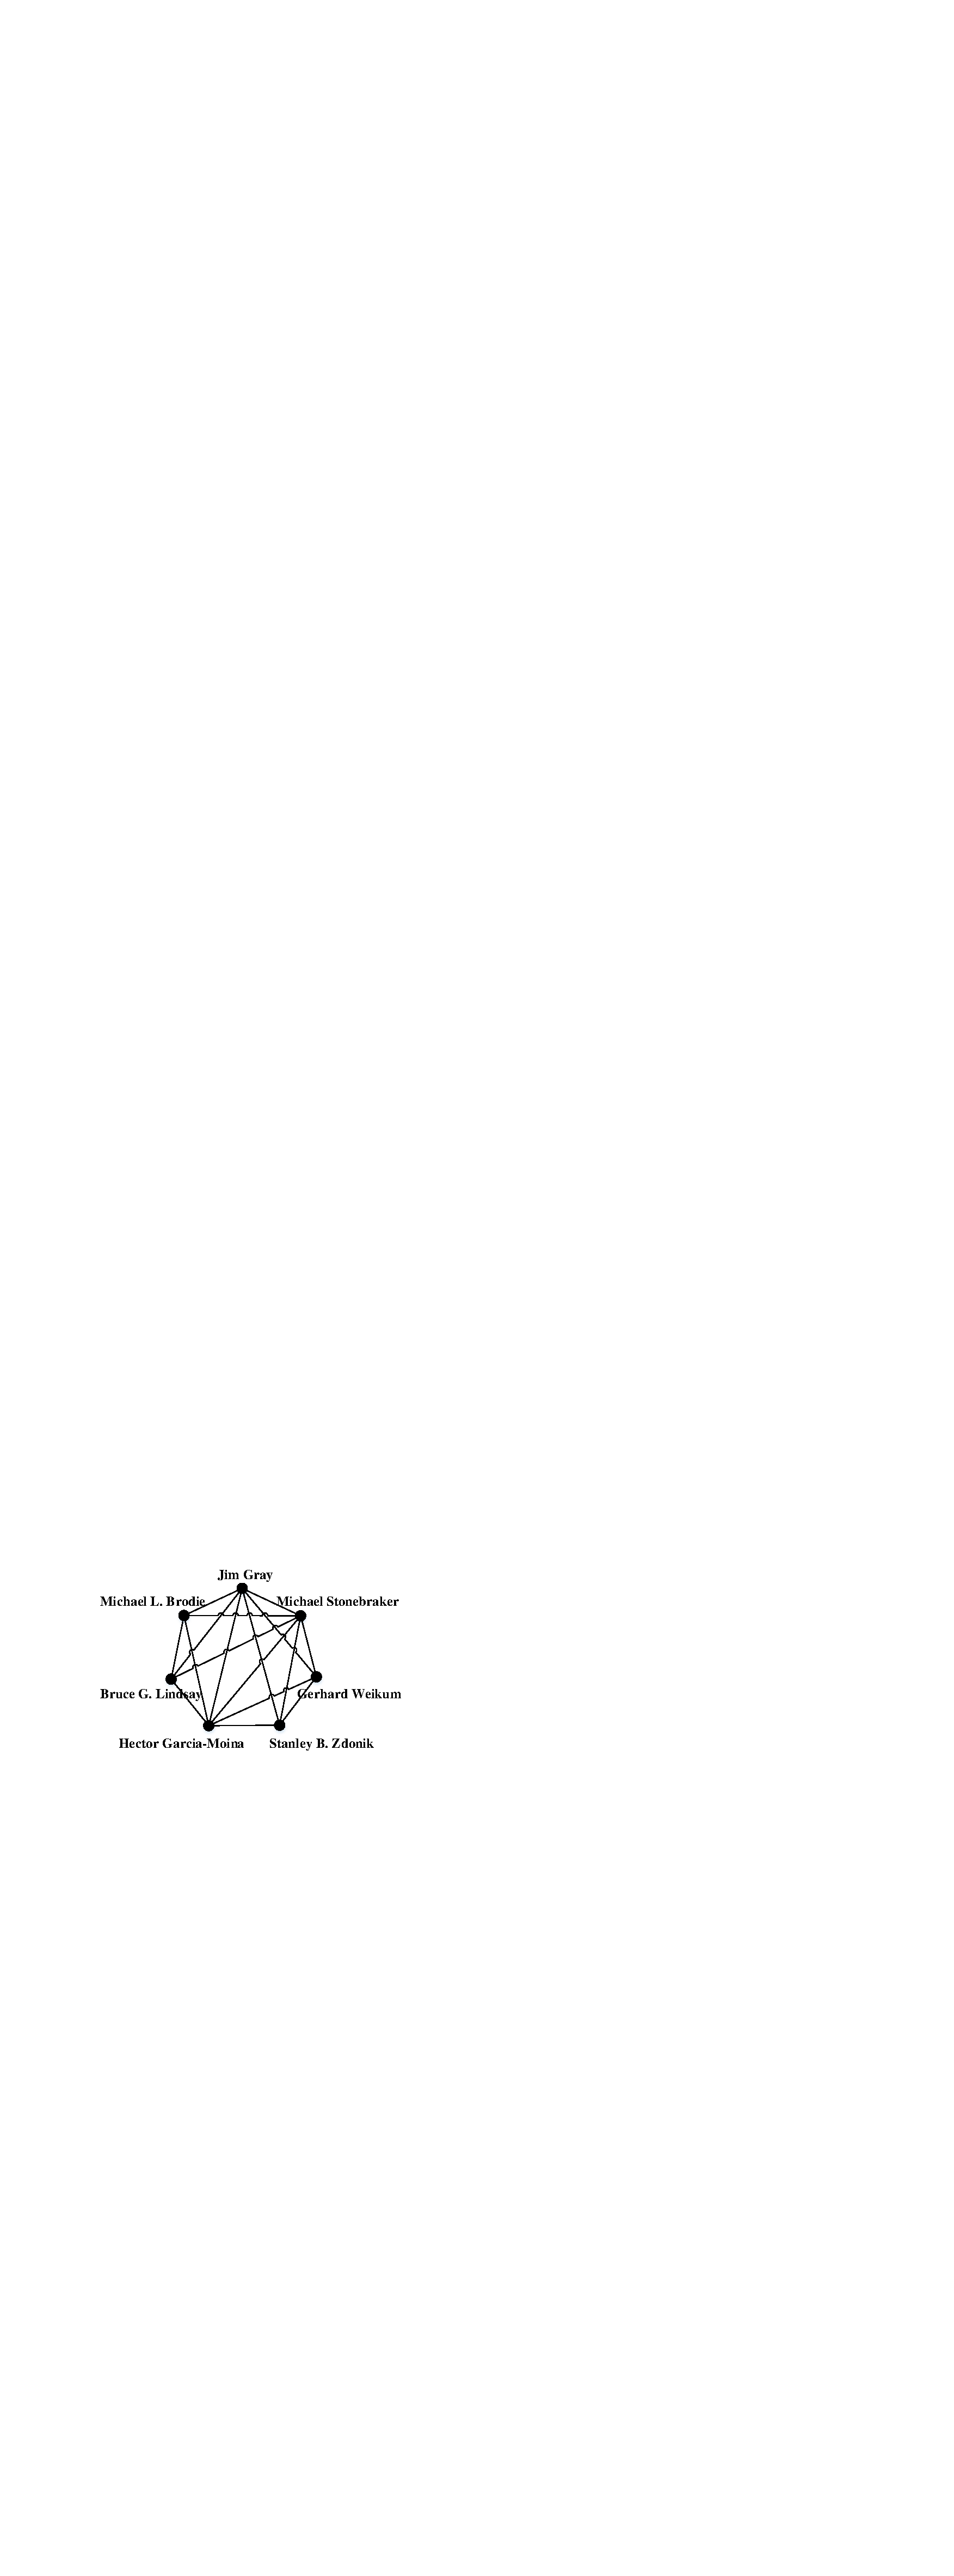
\includegraphics[width=.445\columnwidth]{figures/jim1}
            \label{fig:jim1}
        }
        \hspace{1ex}
        \subfigure[\{sloan, digital, sky, data, sdss\}]{
            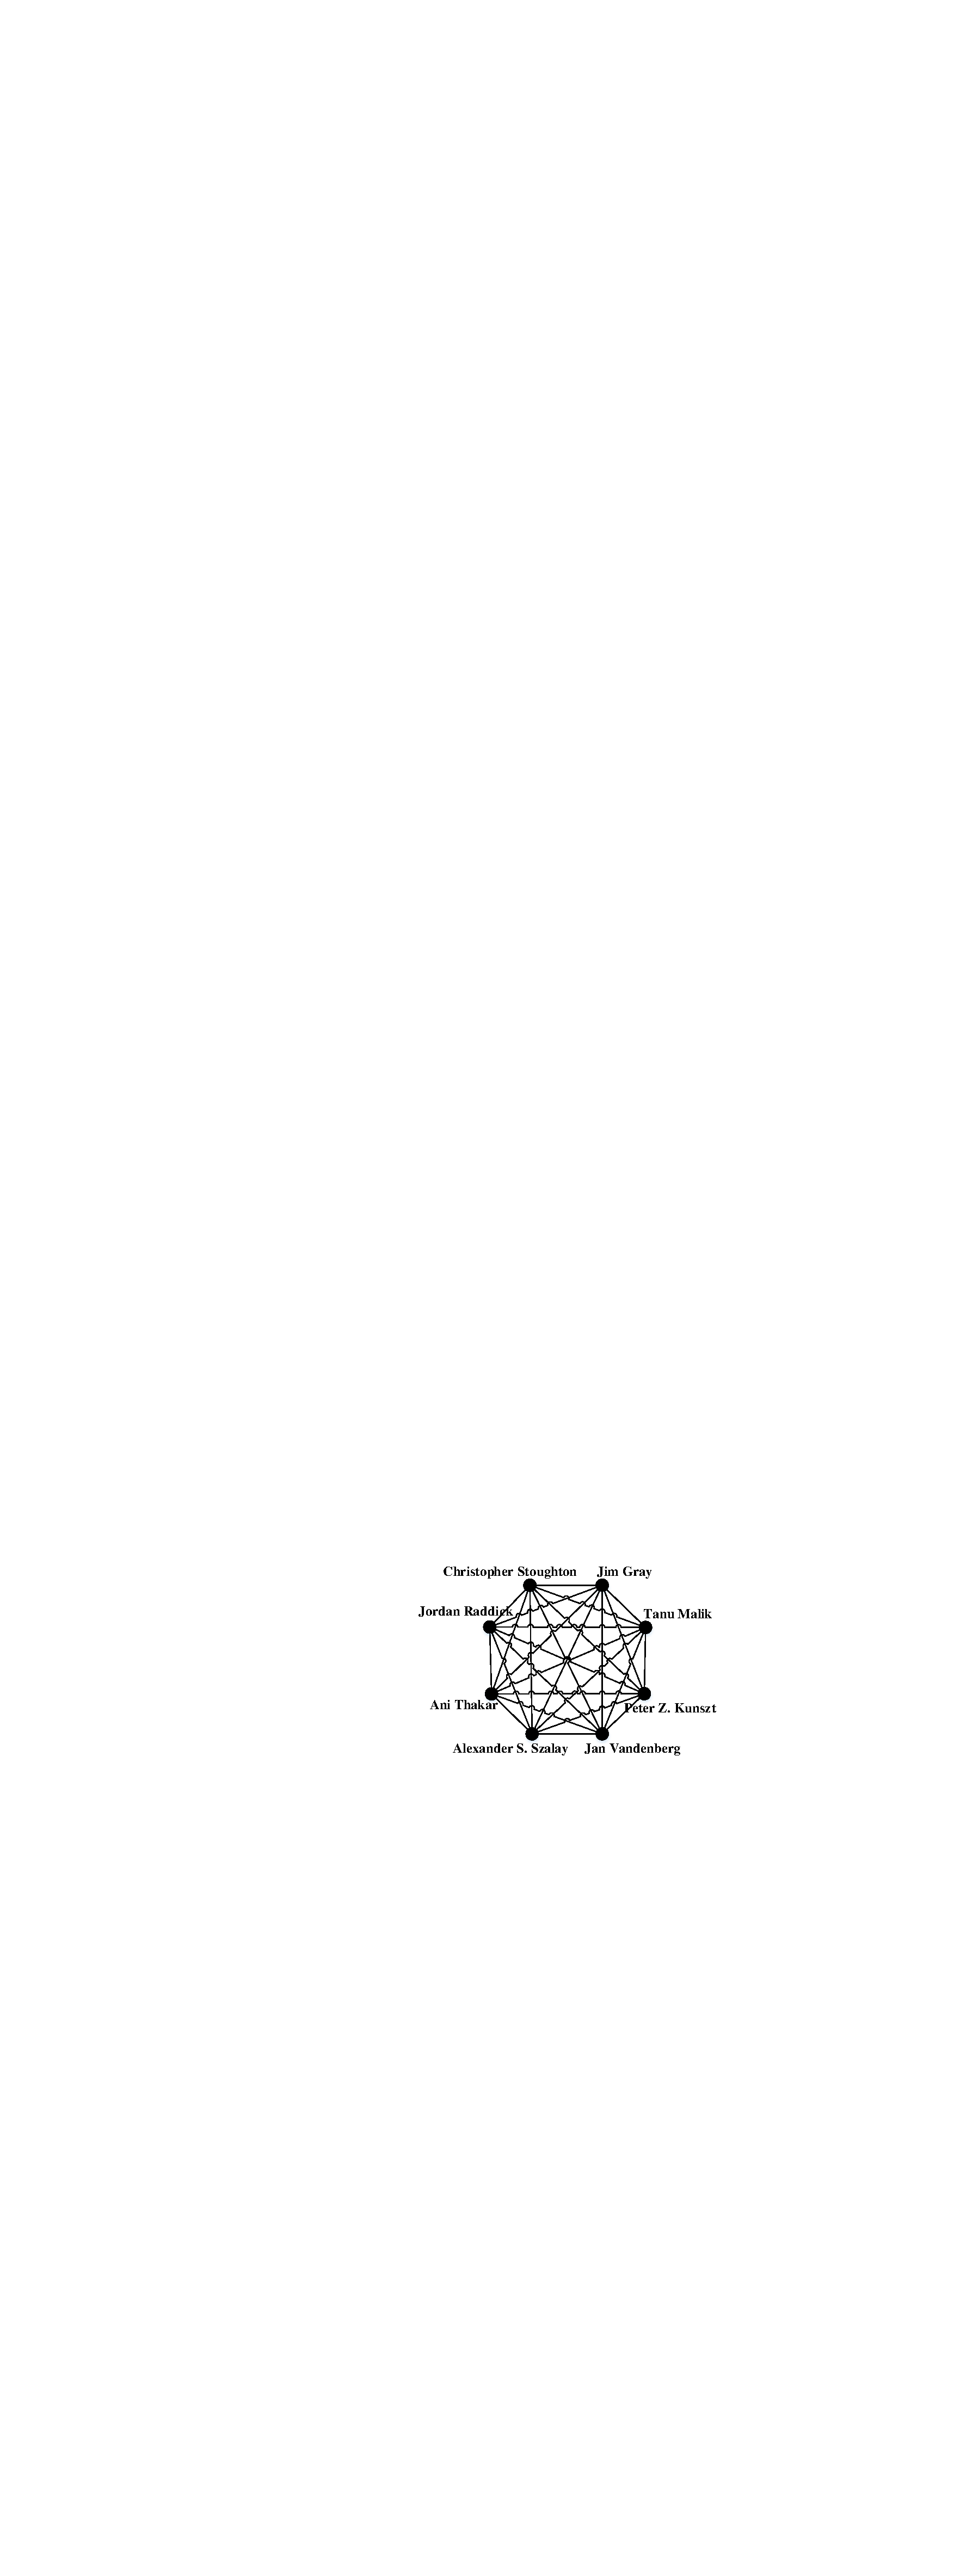
\includegraphics[width=.435\columnwidth]{figures/jim2}
            \label{fig:jim2}
        }
    }
    \caption{Two ACs of Jim Gray (with AC labels).}\label{fig:jim}
\end{figure}

Let us further illustrate the {\it AC search} query on the DBLP bibliographical network, with $q={\tt Jim~Gray}$ and $k=4$ (i.e., the minimal degree of each AC vertex is 4). For discussions, we define the {\it label} of an AC to be a set of keywords that appear in all the vertices of the AC.  Figure~\ref{fig:jim} shows the two ACs found and their respective labels.  We can see that the two ACs contain completely different authors (except Jim himself). Moreover, the label of each AC reflects the backgrounds of the people within that AC (e.g., in Figure~\ref{fig:jim}(a), the 6 researchers connected to Jim are well known for their work in database systems; in Figure~\ref{fig:jim}(b), the 7 scientists linked to Jim are involved in the SDSS (or Sloan Digital Sky Survey) project)~\footnote{URL of the SDSS project: \url{http://www.sdss.org}.}. We have also performed search on $q$ using the existing algorithm~\cite{KDD2010}, and found that the community contains all the 14 vertices shown in Figures~\ref{fig:jim}(a) and (b). The main reasons are: (1) these nodes are all heavily linked to Jim; and (2) vertex keywords are not considered in the community search process. It is not easy from this community to understand which researcher has what kind of collaboration with Jim. In contrast, the AC search places these vertices into two communities, containing vertices that are cohesive in terms of {\it structure} and {\it keyword}. The ACs found allow a user to focus on the important vertices that constitute a community. For example, using the AC of Figure~\ref{fig:jim}(a), a database conference organizer can invite speakers who have a close relationship to Jim. As we will explain later, our AC search solutions use vertex keywords effectively, and are better than existing algorithms~\cite{KDD2010,local2014} that do not use these keywords.

Performing an AC search is not straightforward, since the graph $G$ to be explored can be very large, and the (structure and keyword) cohesiveness criteria for governing the community search are complex. To tackle this challenge, a straightforward way is first to consider all the possible keyword combinations, and then return the subgraphs,
which satisfy the minimum degree constraint and have the most shared keywords.
However, this solution, which requires the enumeration of all the subsets of $q$'s keyword set, has a complexity exponential to the size $l$ of $q$'s keyword set. In our experimental evaluation, for some queries, $l$ can have a value of 30, resulting in the consideration of $2^{30}=1,073,741,824$ subsets of $q$. The algorithm is impractical, especially when $q$'s keyword set is large. We observe the {\it anti-monotonicity} property, which states that given a set $S$ of keywords, if it appears in every vertex of an AC, then for every subset $S'$ of $S$, there exists an AC in which every vertex contains $S'$.
We use this intuition to propose better algorithms. We further develop the \emph{CL-tree}, an index that organizes the vertex keyword data in a hierarchical structure. The CL-tree has a space and construction time complexity linear to the size of $G$. We have developed three different AC search algorithms based on the CL-tree, and they are able to achieve a superior performance.

We have performed extensive experiments on our solutions on four large real graph datasets (namely Flickr, DBLP, Tencent, and DBpedia). We have developed several measures to measure the quality of a community, based on occurrence frequencies of keywords and similarity between the keyword sets of two vertices. We conducted a detailed case study on DBLP. These results confirm the superiority of the AC over the communities returned by existing algorithms, in terms of community quality.
Particularly, compared to two representative algorithms~\cite{KDD2010,local2014}, it is generally easier to understand the meaning behind the ACs;
the label of the AC can tell clearly what the community is about. The performance of our best algorithm is 2 to 3 order-of-magnitude better than solutions that do not use the CL-tree. Another advantage of our approaches is that they organize and search vertex keywords for ACs effectively, achieving a higher efficiency than existing community search solutions (that do not use vertex keywords in the community search process).

As a summary, we propose the AC, which is a new definition of the community that considers both structure and keyword cohesiveness. To perform efficient AC search, we develop the CL-tree and its associated algorithms. We perform experimental evaluation on real graph datasets to validate our approaches.  Notice that although our solutions are developed based on the minimum degree metric in this paper, they can potentially be used to address other definitions of communities (e.g., $k$-truss).  Our study can also inspire the development of better community detection algorithms that take vertex keywords into account.

The rest of our paper is organized as follows. In Section~\ref{problem} we give the problem definition.
Section~\ref{basic} presents the basic solutions, and Section~\ref{index} discusses the CL-tree. We present the query algorithms in Section~\ref{query}. Our experimental results are reported in Section~\ref{experiment}. We review the related work in Section~\ref{related}
and conclude in Section~\ref{conclusion}.
\fi 